\section{Differentitaion}
\label{sec:differentiation}
To characterize the influence of \ac{pdgf} stimulation on \acp{haosmc}, the cells were first treated with \ac{tgf} for four days to push them towards a phenotype that resembles the contractile phenotype. Cells were stimulated for two days from this standardized starting point with \ac{il1} and \ac{pdgf}. The induced phenotypes were then characterized via \ac{qpcr} and Seahorse Assay.

    \subsection{Expression of CNN1 and MMP9}
    \label{subsec:qPCR}
    \begin{figure}[h!]
    \capstart
        \centering
    	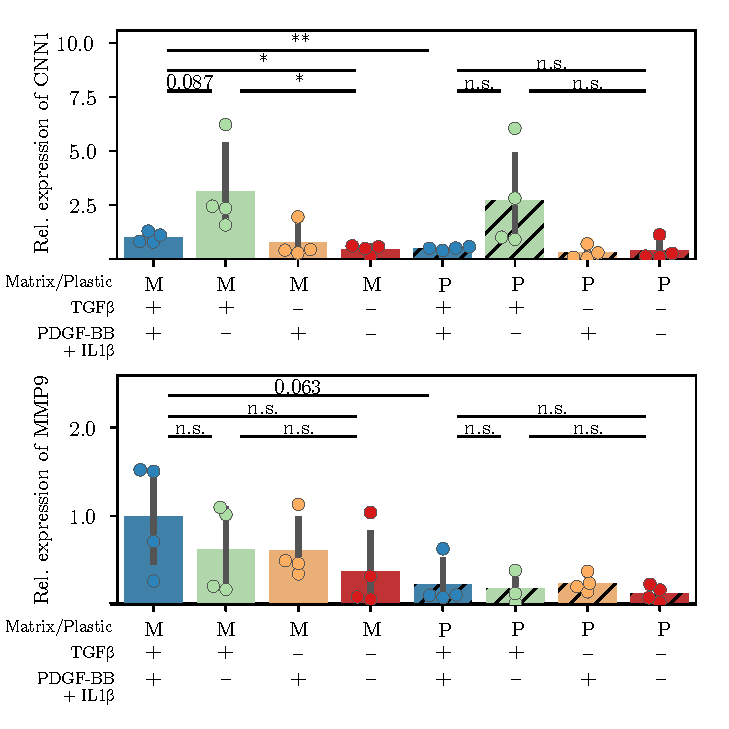
\includegraphics{Abbildung/qPCR.pdf}

    	\begin{minipage}{\captionwidth}
    		\caption[CNN_qPCR]{\uzlemph{Relative Expression of \ac{cnn1} and \ac{mmp9} in \acp{haosmc}} \newline qPCR analysis of expression for contractile marker \ac{cnn1} (top) and synthetic marker \ac{mmp9} (bottom) for \acp{haosmc} differentiated with different combinations of cytokines:
            \textbf{++:} four days with \ac{tgf} followed by two days with \ac{il1} and \ac{pdgf};
            \textbf{+–:} four days with \ac{tgf} followed by two days without stimulation;
            \textbf{–+:} four days without stimulation followed by two days with \ac{il1} and \ac{pdgf};
            \textbf{––:} six days without stimulation.
            All four conditions were tested on two different surfaces (plastic vs. \ac{col1} matrix). Expression levels are in relation to expression of housekeeping gene \ac{gapdh}. Statistical analysis for (n\,=\,4) biological repeats was performed using student's T-test: $*: p < 0.05; **: p < 0.01$}
    		\label{fig:qPCR_result}
    	\end{minipage}
    \end{figure}

    To confirm that the \acp{haosmc} first adopt a contractile phenotype and to track further differentiation after stimulation with \ac{pdgf}, the \ac{mRNA} levels of the marker genes \ac{cnn1} and \ac{mmp9} were determined using \ac{qpcr}. \ac{cnn1} serves as a contractile marker and \ac{mmp9} as a marker for a synthetic phenotype. For better comparability, \ac{mRNA} levels were normalized with the expression of the housekeeping gene \ac{gapdh}.\\
    Figure \ref{fig:qPCR_result} (top panel) illustrates that stimulation of \acp{haosmc} cultivated on a \ac{col1}-matrix with \ac{tgf} causes a significant increase in \ac{cnn1} expression (+– vs. – –). After further stimulation with \ac{pdgf} and \ac{il1}, while not significant, \ac{cnn1} expression declines again (+– vs. ++) but is still significantly higher than in \acp{haosmc}, which were not stimulated (– – vs. ++). A similar trend is noticeble for \acp{haosmc} cultivated on plastic. However, this effect did not reach significance after four biological repeats. Additionally, stimulation of \acp{haosmc} on plastic with \ac{tgf}, followed by stimulation with \ac{pdgf} and \ac{il1}, yields a significantly lower expression of \ac{cnn1} (++ Matrix vs. ++ Plastic).\\
    As seen in the bottom panel of figure \ref{fig:qPCR_result} no statistically significant trends can be observed after four biological repeats for the expression of \ac{mmp9}. Still, the average expression of \ac{mmp9} seems to increase on \ac{col1} matrix compared to plastic for all conditions. The most notable difference being between \acp{haosmc} treated first with \ac{tgf} as well as with \ac{pdgf} and \ac{il1} (++ Matrix vs. ++ Plastic, p\,=\,0.063).


    \subsection{Energy profile}
    \label{subsec:energy}
    In addition to the expression of \ac{cnn1} and \ac{mmp9}, the energy profiles of \acp{haosmc} were assessed via Seahorse Assay. It is important to note that the assay was carried out on plastic because the \ac{col1} matrix does not fit into the confined compartment created by the piston to record the \ac{ocr} and \ac{ecar}. Furthermore, only two biological repeats were evaluated because it became clear that all other experiments would be carried out on a \ac{col1} matrix. Therefore all the following considerations should take these decisions and limitations into account.

    \begin{figure}[h!]
    \capstart
        \centering
        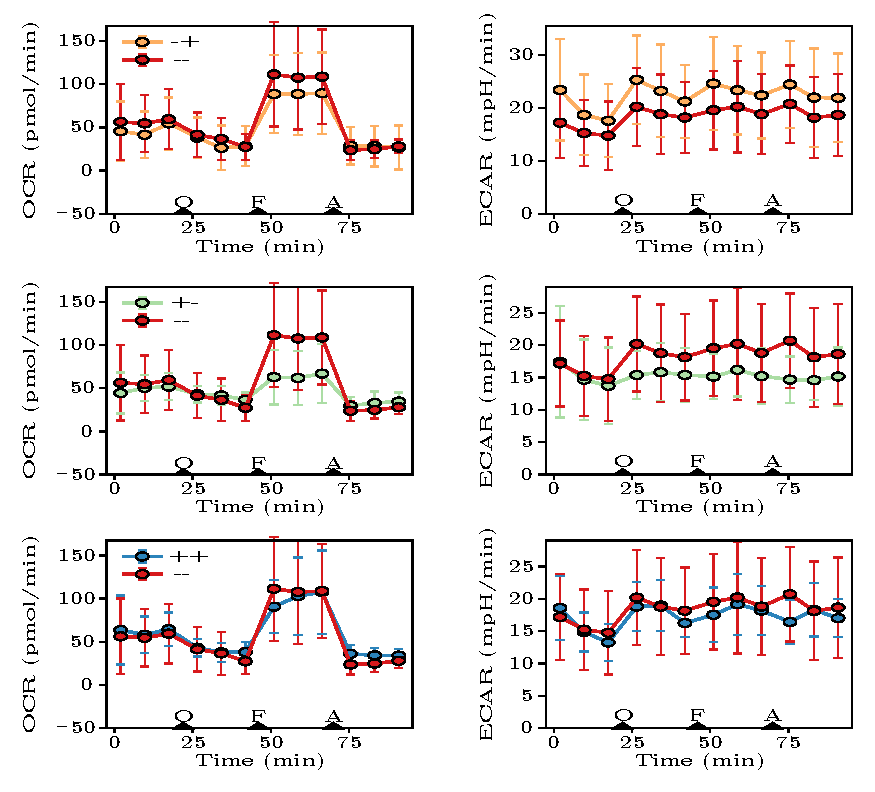
\includegraphics{Abbildung/Seahorse_tracks.pdf}

        \begin{minipage}{\captionwidth}
            \caption[seahorse_tracks]{\uzlemph{\ac{ocr} and \ac{ecar} of \acp{haosmc}} \newline Seahorse assay for \acp{haosmc} differentiated with different combinations of cytokines.
            \textbf{++:} four days with \ac{tgf} followed by two days with \ac{il1} and \ac{pdgf};
            \textbf{+–:} four days with \ac{tgf} followed by two days without stimulation;
            \textbf{–+:} four days without stimulation followed by two days with \ac{il1} and \ac{pdgf};
            \textbf{––:} six days without stimulation.
            \ac{ocr} and \ac{ecar} are shown for –+ (top), +– (middle) and ++ (bottom) compared to ––. Injection times for toxins (O: Oligomycin; F: FCCP; A: Antimycin A) are marked as triangles. All tracks were recorded for cells cultivated on plastic. Shown datapoints are the average of (n\,=\,2) biological repeats.
            }
            \label{fig:seahorse_tracks}
        \end{minipage}
    \end{figure}

    The readout parameters of the Seahorse assay are the \ac{ocr} as a representation of mitochondrial activity and the \ac{ecar}, representing the glycolytic activity of the cells. \ac{ocr} and \ac{ecar} for \acp{haosmc} are displayed in figure \ref{fig:seahorse_tracks}. All cells show characteristic changes in \ac{ocr} after the addition of toxins impacting the respiratory chain (compare to figure \ref{fig:seahorse_basics} B). After inhibition of the \ac{atp} synthase with Oligomycin, the basal \ac{ocr} drops, revealing the proportion of the \ac{ocr} required for \ac{atp} production. Subsequently, the addition of \ac{fccp} decouples the respiratory chain, destroying the proton gradient over the mitochondrial membrane. As a result, the cells reach their maximal respiratory capacity. Finally, the inhibition of coenzyme Q-cytochrome c reductase (complex III) with Antimycin A stops all mitochondrial respiratory activity.\\
    The \ac{ecar} shows a mild increase for all conditions after adding of Oligionmycin, most likely because the cells compensate for the loss of mitochondrial \ac{atp} production via increased glycolysis.

    \begin{figure}[h!]
    \capstart
        \centering
    	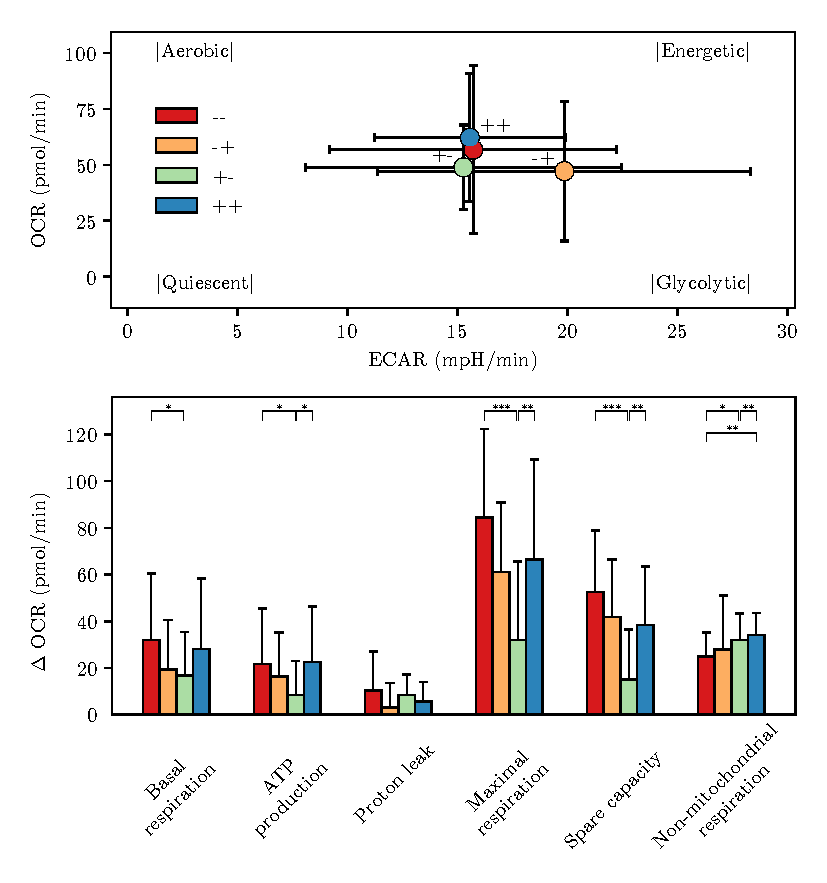
\includegraphics{Abbildung/Seahorse_summary_merged.pdf}

    	\begin{minipage}{\captionwidth}
    		\caption[energy_profile]{\uzlemph{Energy profile of \acp{haosmc}} \newline Seahorse assay for \acp{haosmc} differentiated with different combinations of cytokines as described in figure \ref{fig:seahorse_tracks}.
            (\textbf{A}) Initial \ac{ocr} and \ac{ecar} of the four tested conditions. (\textbf{B}) Characteristics of the respiratory chain calculated from the tracks shown in figure \ref{fig:seahorse_tracks} as described in section \ref{sec:seahorse}. Statistical analysis for (n\,=\,2) biological repeats was performed using student's T-test: $*: p < 0.05; **: p < 0.01, ; ***: p < 0.001$}
    		\label{fig:energy_profile}
    	\end{minipage}
    \end{figure}

    Looking at the energy profile, which describes the basal state of the differentiated cells, \ac{ocr} and \ac{ecar} are quite similar for the conditions ++, +–, and ––. The only outlier showing a higher \ac{ecar} are \acp{haosmc} only stimulated with only \ac{il1} and \ac{pdgf} (–+) (fig. \ref{fig:energy_profile}, A). More interesting differences can be observed when examining the characteristics of the respiratory chain. Stimulation with only \ac{tgf} causes a significant decrease in basal respiration, \ac{atp} production, maximal respiration, and spare capacity (figure \ref{fig:energy_profile}, B top). Further stimulation with \ac{il1} and \ac{pdgf} then causes a significant increase of these parameters to similar levels as in initially dedifferentiated \acp{haosmc} (figure \ref{fig:energy_profile}, B bottom).

\section{Evaluation of oxidative Stress}
\label{sec:oxStress}
Finally, it was evaluated if further stimulation with \ac{pdgf} would stimulate the cells to generate \ac{ros} to the extent that can not be compensated by the \ac{ros} defense and lead to oxidative stress.

    \subsection{PDGF boost of out cells induces oxidative stress}

    \begin{figure}[h!]
    \capstart
        \centering
    	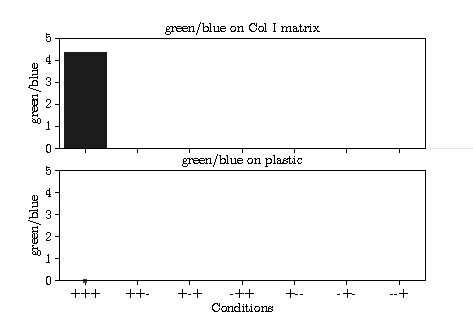
\includegraphics{Abbildung/CellROX_initial_cond.pdf}

    	\begin{minipage}{\captionwidth}
    		\caption[repeat_Lisa]{\uzlemph{Boost with \ac{pdgf} induces the generation of \ac{ros}.} \newline CellROX\texttrademark~assay for \acp{haosmc} differentiated with different combinations of cytokines: four days with \ac{tgf}; followed by two days with \ac{il1} and \ac{pdgf}; followed by 2\,h boost with 200\,ng/mL \ac{pdgf}. Differentiation and assay carried out on \ac{col1} matrix (top) or plastic (bottom). The hown signal was calculated according to section \ref{subsec:cellrox_data_processing} as the CellROX\texttrademark~Green signal, normalized by Hoechst 33342 signal. No statistical analysis for (n\,=\,1) biological repeats was performed. }
    		\label{fig:cellrox_8con}
    	\end{minipage}
    \end{figure}

    At first, an experiment already done in the group was validated. Stimulating the four tested combinations for 2 additional hours with 200\,ng/mL \ac{pdgf} in \ac{hbss}. As displayed in figure \ref{fig:cellrox_8con}, only stimulation for four days with \ac{tgf}, followed by two days with \ac{il1} and \ac{pdgf}, followed by a 2\,h boost with \ac{pdgf}, triggered noticeable \ac{ros} generation for cells cultivated on \ac{col1}-matrix. No generation of \ac{ros} was detectable for \acp{haosmc} cultivated without the \ac{col1}-matrix.

    \subsection{Characterization of the CellROX\texttrademark~Assay}
    \begin{figure}[h!]
    \capstart
        \centering
    	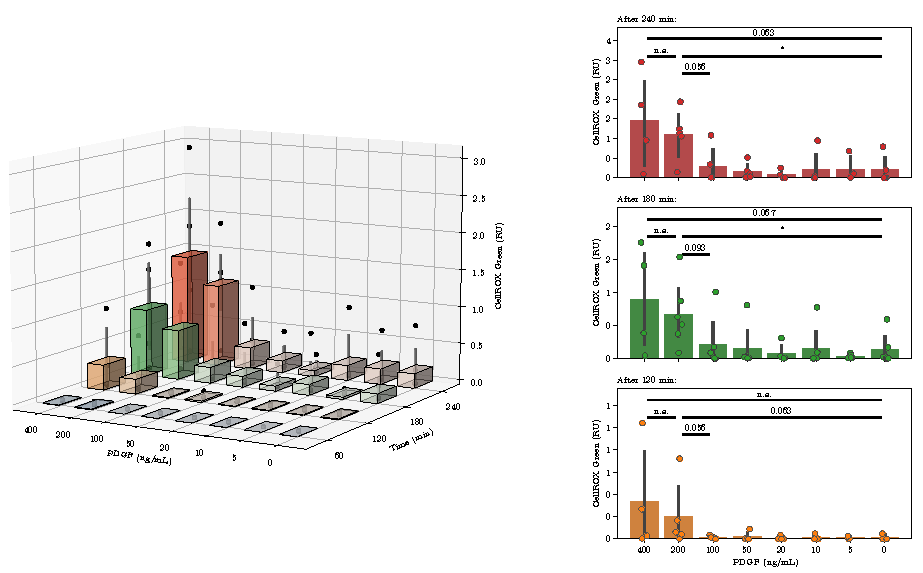
\includegraphics{Abbildung/CellROX_titration_no_norm.pdf}

    	\begin{minipage}{\captionwidth}
    		\caption[cellROX_titration]{\uzlemph{\ac{pdgf} boost titration} \newline
            CellROX\texttrademark~assay for \acp{haosmc} differentiated with different combinations of cytokines: four days with \ac{tgf}; followed by two days with \ac{il1} and \ac{pdgf}; followed by 4\,h boost with 0\,-\,400\,ng/mL \ac{pdgf}. Differentiation and assay carried out on \ac{col1} matrix.
            (\textbf{A}) 3D visualization: CellROX\texttrademark~Green signal as a function of \ac{pdgf} concentration during the boost as well as incubation time.
            (\textbf{B}) 2D visualization: CellROX\texttrademark~Green signal as a function of \ac{pdgf} concentration after 120 min, 180 min and 240\,min.
            The shown signal was calculated according to section \ref{subsec:cellrox_data_processing} as the CellROX\texttrademark~Green signal, normalized by Hoechst 33342 signal. Statistical analysis for (n\,=\,6) biological repeats was performed using Mann-Whitney U test: $*: p < 0.05; **: p < 0.01$. Note that not every biological repeat covered \textit{all} \ac{pdgf} concentration. }
    		\label{fig:cellROX_titration}
    	\end{minipage}
    \end{figure}

    To get a better understanding of the assay and its limits, a titration was carried out. For this, \acp{haosmc} stimulated for four days with 5\,ng/mL \ac{tgf} as well as two days with 10\,ng/mL \ac{il1} and 10\,ng/mL  \ac{pdgf}, were boosted with different concentrations of \ac{pdgf} (0\,-\,400\,ng/mL). Signal was detected after 60, 120, 180, and\,240 min in \ac{hbss}. As seen in figure \ref{fig:cellROX_titration}, the CellROX\texttrademark~Green signal is negligible after 60\,min and then increases with elongated boost times. Moreover, CellROX\texttrademark~Green signal stays negligible for boost concentrations < 100\,ng/mL \ac{pdgf}. After 180 and 240\,min (figure \ref{fig:cellROX_titration} B top and middle), CellROX\texttrademark~Green signal is significantly increased for boost with 200\,ng/mL \ac{pdgf} compared to no boost (0\,ng/mL \ac{pdgf}). While the signal in wells boosted with 400\,ng/mL \ac{pdgf} was, on average higher than the signal after boost with 200\,ng/mL \ac{pdgf}, this increase was not reproducible. On one hand, the signal was extremely high. On other hand, the other two repeats, it collapsed.

    \begin{figure}[h!]
    \capstart
        \centering
    	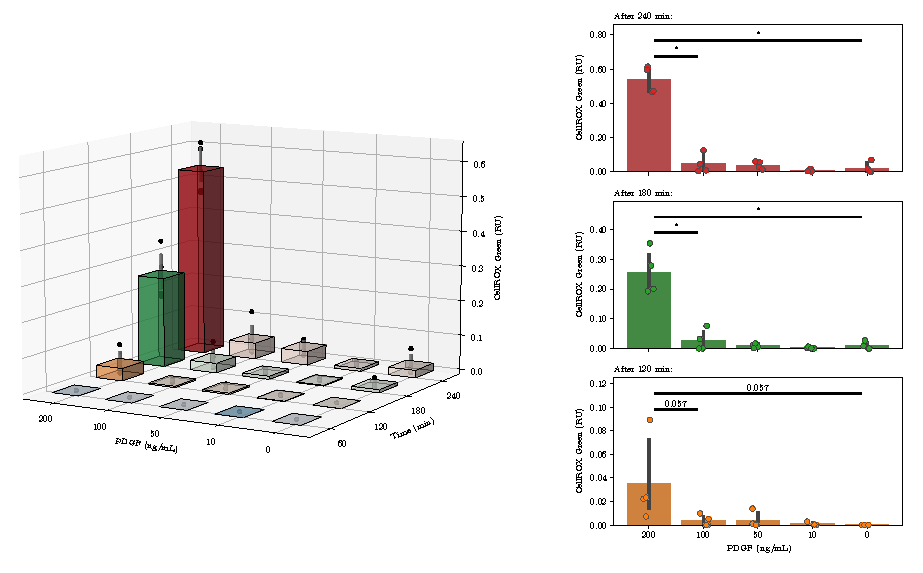
\includegraphics{Abbildung/CellROX_titration_norm.pdf}
    	\begin{minipage}{\captionwidth}
    		\caption[cellROX_titration_norm]{\uzlemph{\ac{pdgf} boost titration - normalized} \newline
            CellROX\texttrademark~assay for \acp{haosmc} differentiated with different combinations of cytokines: four days with \ac{tgf}; followed by two days with \ac{il1} and \ac{pdgf}; follwoed by 4\,h boost with 0\,-\,200\,ng/mL \ac{pdgf}. Differentiation and assay carried out on \ac{col1} matrix.
            (\textbf{A}) 3D visualization: CellROX\texttrademark~green signal as a function of \ac{pdgf} concnentration during the boost as well as incubation time.
            (\textbf{B}) 2D visualization: CellROX\texttrademark~green signal as a function of \ac{pdgf} concnentration after 120\,min, 180\,min and 240\,min.
            Shown signal was calculated according to section \ref{subsec:cellrox_data_processing} as the CellROX\texttrademark~Green signal, normalized by Hoechst 33342 signal, further the signal was normalized via the total signal of the biological repeat. Statistical analysis for (n\,=\,4) biological repeats was performed using Mann-Whitney U test: $*: p < 0.05; **: p < 0.01$.}
    		\label{fig:cellROX_titration_norm}
    	\end{minipage}
    \end{figure}

    Overall, the trend of greatly increased CellROX\texttrademark~signal for a boost with 100 or 200\,ng/mL \ac{pdgf} was consistent within biological repeats; however, the variance between repeats was almost as high as the differences between the conditions. Potential causes for this phenomenon are discussed in section \ref{link to the discussion when I write it}. To account for this large variation between biological repeats, the assay was reevaluated by the selection of shared conditions among the biological repeats normalized to the cumulative intensity of all conditions of the biological repeat (see figure \ref{fig:cellROX_titration_norm}). This step compensates for differences between biological repeats. The interpretation of the results remains unaffected by normalization: CellROX\texttrademark~Green signal after 180 and 240\,min is significantly higher for cells boosted with 200\,ng/mL \ac{pdgf} than cells that were not boosted (0\,ng/mL \ac{pdgf}).

    \subsection{Rescue of ROS production using NAC}
        \begin{figure}[h!]
    \capstart
        \centering
    	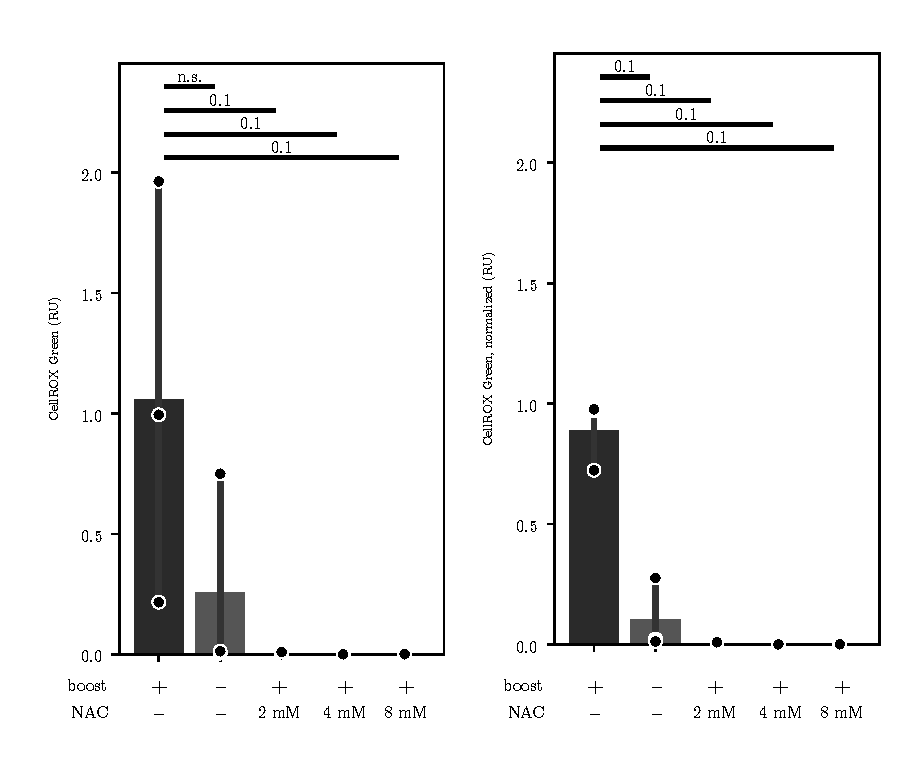
\includegraphics{Abbildung/NAC_quench.pdf}

    	\begin{minipage}{\captionwidth}
    		\caption[NAC quench]{\uzlemph{\ac{ros} generation due to \ac{pdgf} boost can be rescued with \ac{nac}} \newline
            CellROX\texttrademark~assay for \acp{haosmc} differentiated with different combinations of cytokines: four days with \ac{tgf}; followed by two days with \ac{il1} and \ac{pdgf}; followed by 3\,h boost with 200\,ng/mL \ac{pdgf}. Differentiation and assay carried out on \ac{col1} matrix. Cells were treated with 2, 4, or 8\,mM of \ac{nac} 2\,h before the assay.
            Shown signal was calculated according to section \ref{subsec:cellrox_data_processing} as the CellROX\texttrademark~Green signal, normalized by Hoechst 33342 signal (\textbf{A}), further the signal was normalized via the total signal of the biological repeat (\textbf{B}). Statistical analysis for (n\,=\,4) biological repeats was performed using Mann-Whitney U test: $*: p < 0.05; **: p < 0.01$.
            pos Ctrl: not treated with \ac{nac}, negCtrl: no boost with \ac{pdgf}}
    		\label{fig:NAC_quench}
    	\end{minipage}
    \end{figure}

Finally, a rescue experiment was performed to verify that the observed signal in the CellROX\texttrademark~assay was due to the generation of \ac{ros}. \ac{ros} generation was quenched by adding of 2,\,4,\,or 8\,mM of \ac{nac}. Indeed, a clear trend can be observed: \acp{haosmc} treated with \ac{nac} showed no signal. However, this trend remained statistically insignificant for triplicates.\\
It is noteworthy that the signal only builds up over 15\,-\,20\,min under the microscope after the cells were taken out of the incubator. This observation indicates that the generation of \ac{ros} might not be exclusively triggered by \ac{pdgf} boost. However, it could also require additional contributors like the loss of the optimized atmosphere of 37°C and 5\,\% \ac{co2} in the incubator. This fact might not have surfaced during the titration assay because cells were taken out of the incubator after one hour to image them for the first time.

\section{Database and GWAS Navigator}

    \subsection{Curation of Data}

    \begin{table}[h!]
    \capstart
    \centering
    \begin{minipage}{\captionwidth}
        \caption[db tables]{\uzlemph{List of Database Tables}\newline
    List of all the datasets and corresponding tables which were funneled into the database. For primary keys, foreign keys as well as fields on which an idex exists, please consulte figure \ref{fig:db_er}. The size of the tables (and accompanying indices) is indicated by the number of databank pages that are reserved for the data, each page fitting 4096 bytes.}
        \label{tab:db_tables}
    \end{minipage}
        \begin{tabular}{l|l|r}
        Data                                       & Tables                             & Page count\newline (including indices)                                                                      \\ \hline
        \multirow{3}{*}{GWAS Summary stats}        & variation                          & 418,318                                                                                              \\
                                                   & gwas\_meta\_cad                    & 867,025                                                                                              \\
                                                   & identified\_proxy\_SNPs\_tbl       & 4                                                                                                   \\ \hline
        \multirow{2}{*}{HGNC gene list}            & hgnc\_all\_symbols\_tbl            & 826                                                                                                 \\
                                                   & hgnc\_approved\_symbols\_tbl       & 592                                                                                                 \\ \hline
        \multirow{3}{*}{Linked SNPs}               & linked\_SNPs\_tbl                  & 8,819                                                                                                \\
                                                   & population\_tbl                    & 1                                                                                                   \\
                                                   & consequence\_tbl                   & 1                                                                                                   \\ \hline
        \multirow{2}{*}{Ensembl Genome Annotation} & ensembl\_genelist\_tbl             & 613                                                                                                 \\
                                                   & ensembl\_genelist\_biotypes\_tbl   & 1                                                                                                   \\ \hline
        \multirow{2}{*}{Ensembl Regulatory Build}  & ensembl\_reg\_build\_tbl           & 8,778                                                                                                \\
                                                   & ensembl\_reg\_build\_features\_tbl & 1                                                                                                   \\ \hline
        TSS                                        & tss\_tbl                           & 481                                                                                                 \\ \hline
        Open Target Genetics Scores                & opentarget\_l2g\_tbl               & 40,984                                                                                               \\ \hline
        \multirow{2}{*}{GWAS catalog}              & gwascatalog\_associations\_tbl     & 10,569                                                                                               \\
                                                   & gwascatalog\_studies\_tbl          & 326                                                                                                 \\ \hline
        \multirow{2}{*}{TADs}                      & tad\_tbl                           & 902                                                                                                 \\
                                                   & tad\_sample\_tbl                   & 1                                                                                                   \\ \hline
        \multirow{2}{*}{scATAC seq textcite\{\}}   & clint\_miller\_tbl                 & 12,370                                                                                               \\
                                                   & clint\_miller\_biotypes\_tbl       & 1                                                                                                   \\ \hline
        \multirow{2}{*}{scATAC seq CATlas}         & catlas\_tbl                        & 308,574                                                                                              \\
                                                   & catlas\_biotypes\_tbl              & 3                                                                                                   \\ \hline
        \multirow{4}{*}{ABC model}                 & abc\_tbl                           & 153,920                                                                                              \\
                                                   & abc\_targetgenes\_tbl              & 84                                                                                                  \\
                                                   & abc\_celltypes\_tbl                & 3                                                                                                   \\
                                                   & abc\_classes\_tbl                  & 1                                                                                                   \\ \hline
        \multirow{2}{*}{ENCODE cCREs}              & ENCODE\_CCRE                       & 4,451,476                                                                                             \\
                                                   & ENCODE\_CCRE\_META                 & 107                                                                                                 \\ \hline
        total                                      & -                                  & 6,284,781 ($\approx$ 25.75 GB)
        \end{tabular}
    \end{table}

    The first step toward visualization of \ac{gwas} summary statistics was curating of relevant complementary data. Datasets from diverse data sources were downloaded and funneled into an SQLite3 database as described in section \ref{sec:database}. A \ac{sql} database is a two-dimensional relational database that allows easy and fast access to the data for visualization purposes. The data types and their applications are briefly described in section \ref{sec:bioinformatics}. All database tables and their sizes are summarized in table \ref{tab:db_tables}. The relationships between the tables and fields serving as a primary key, foreign, or fields on which an index exists are summarised in the database's \ac{er} diagram in figure \ref{fig:db_er}.

    \begin{figure}[h!]
    \capstart
        \centering
        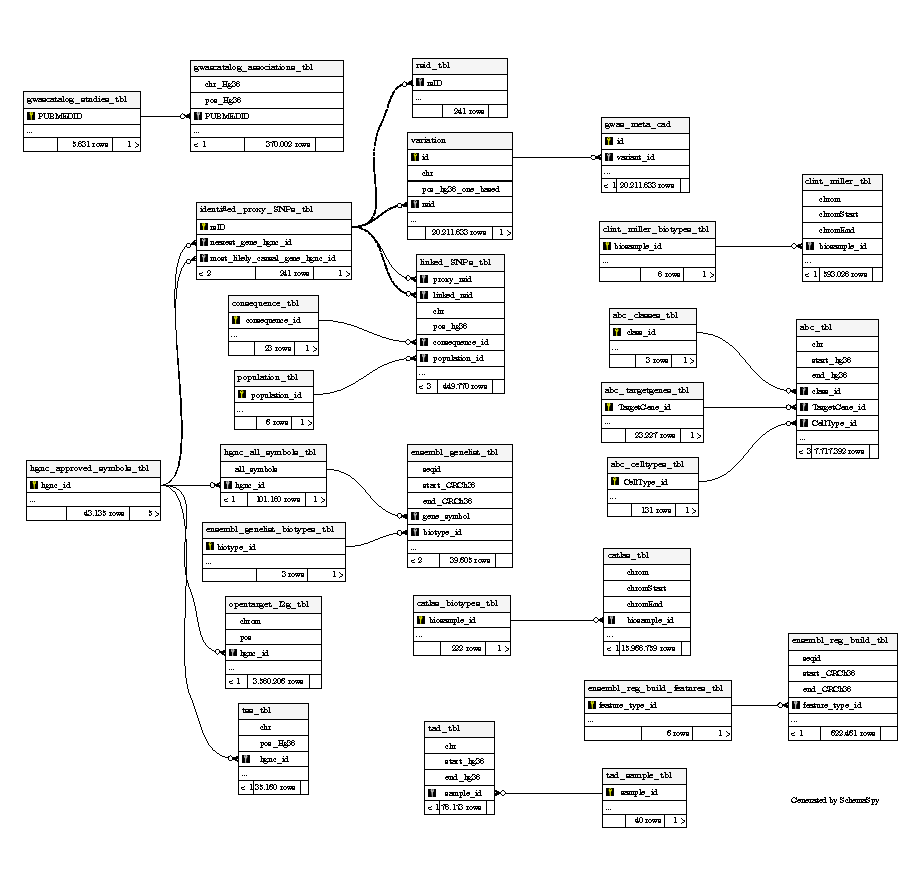
\includegraphics{Abbildung/db-schema.pdf}

        \begin{minipage}{\captionwidth}
            \caption[database]{\uzlemph{Entity-Relationship Diagram of the Database}\newline
            Fields and relationships of the tables listed in table \ref{tab:db_tables}. On spelled out columns an index exists or they are primary or forgein keys. The diagram was generated via SchemaSpy.}
            \label{fig:db_er}
        \end{minipage}
    \end{figure}

    \begin{figure}[H]
        \vspace*{-0.5cm}
        \capstart
        \centering
        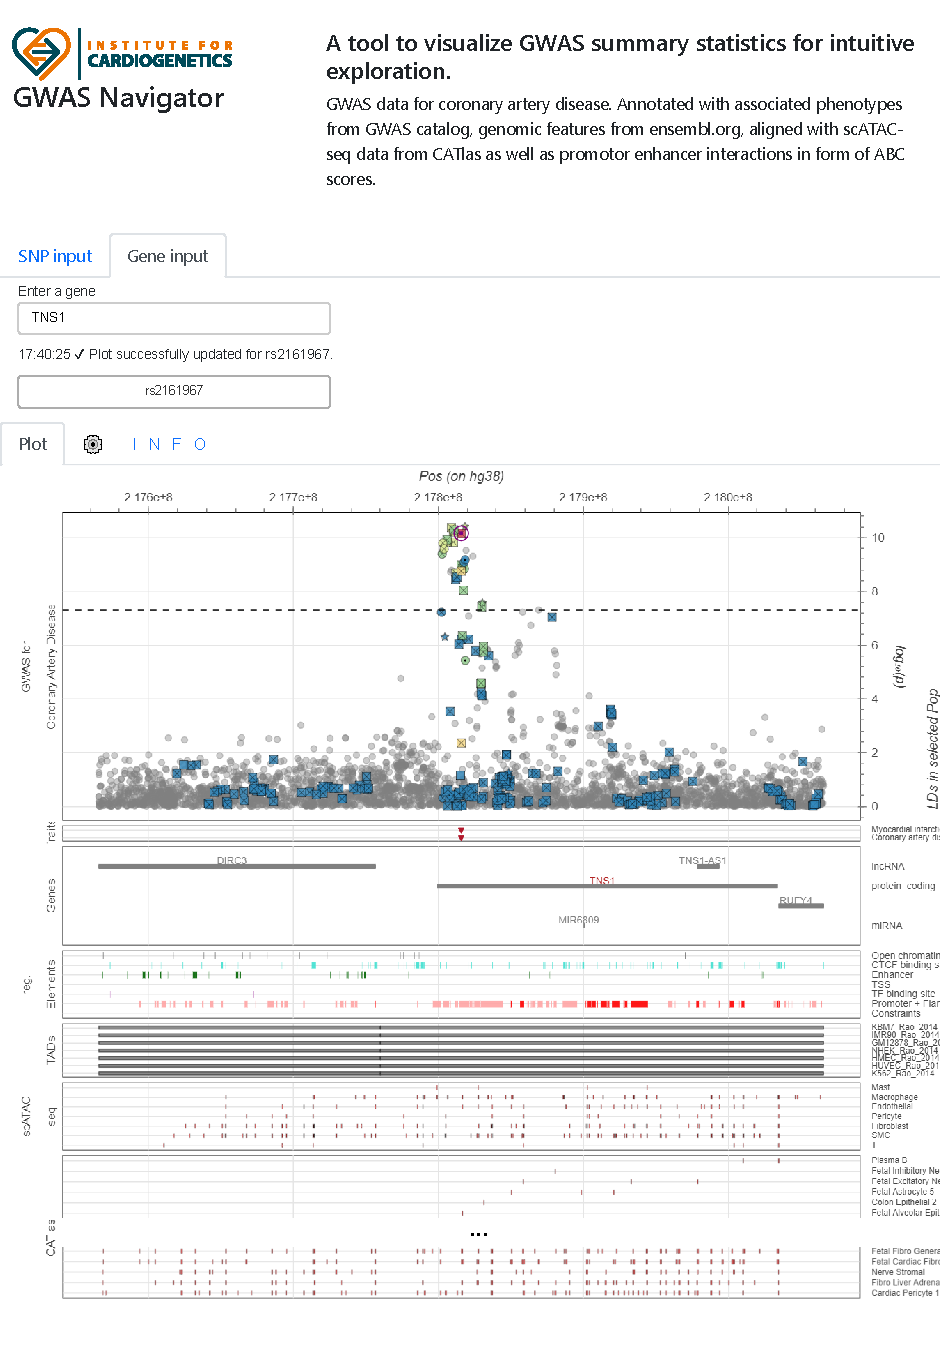
\includegraphics{Abbildung/GWAS_navigator_screenshot.pdf}

        \begin{minipage}{\captionwidth}
            \caption[database]{\uzlemph{The \ac{gwas} Navigator}\newline
            General content of the \ac{gwas} Navigator. The tool contains a manhattan plot with \ac{gwas} summary statistics, containing an additional annotation for variants that are in \ac{ld} with the variant central to the analysis. Further variants identified as proxy variants for other phenotypes are included. Finally, the data are aligned with genomic elements such as genes, regulatory elements, \ac{sc}\ac{atac} data as well as the \ac{abc} model. More details can be assessed by a hover effect as shown in figure \ref{fig:GWAS_navigator_hover}.}
            \label{fig:navigator}
        \end{minipage}
    \end{figure}

    \subsection{Visualization}
    \label{subsec:result_vis}
    Implementing the initially intended use case for the data, a visualization tool for \ac{gwas} summary statistics was built according to section \ref{sec:gwas_vis}. As shown in figure \ref{fig:navigator}, the \ac{gwas} Navigator consists of a separate search bar with a field to specifically search for variants by their rsID and a field that allows searching for genes by their symbol. If the searched gene is associated with one of the proxy variants in \textcite{aragamDiscoverySystematicCharacterization2021}, the tool returns a list of these variants. Else the tool returns the most significant variant in the proximity of the searched gene. After a variant was chosen, the tool displays the \ac{gwas} summary statistics in a 500 kb window centered around the selected variant to the output panel. \ac{gwas} summary statistics are visualized as a zoomed-in Manhatten plot, showing the position of a variant on \ac{hg38} on the x-axis and its p-value on the y-axis. $r^2$ values of variants in \ac{ld} are color-coded. In addition, the most severe consequence for all linked variants predicted by \ac{vep} is indicated by the type of glyph. The \ac{maf} and effect size (\beta) are included in the hover overlay (figure \ref{fig:GWAS_navigator_hover} A). Below this plot, variant trait associations from the \ac{gwas} catalog are indicated for variants that are in \ac{ld} with the variant central to the analysis (figure \ref{fig:GWAS_navigator_hover} B). Furthermore, the region is aligned with protein-coding genes, \acp{lncRNA} and \acp{miRNA} annotated in Ensembl. The names of genes that are associated with the variant of interest (open target genetics \ac{l2g} score > [FIND THE THRESHHOLD]) are labeled in red. In addition, regulatory elements from the Ensembl regulatory build are displayed. Finally, sc\ac{atac} data and enhancers-promotor links from the \ac{abc} model were aligned, automatically hiding tracks with no elements in the visualized region.\\
    The \ac{gwas} Navigator also has a settings tab where individual tracks can be hidden.

    \begin{figure}[h!]
    \capstart
        \centering
        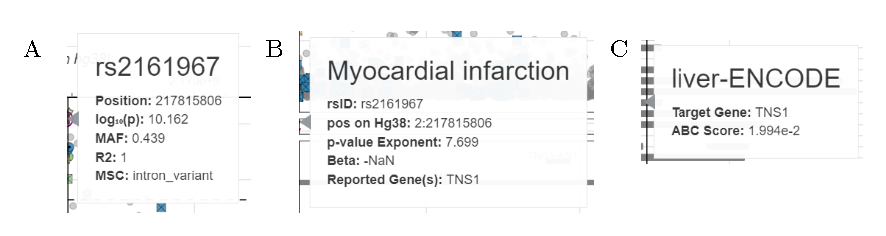
\includegraphics{Abbildung/GWAS_navigator_hover.pdf}

        \begin{minipage}{\captionwidth}
            \caption[database]{\uzlemph{The \ac{gwas} Visualizer - Hovereffect}\newline
            Exampalry hover effects for features displayed in the \ac{gwas} Navigator. (\textbf{A}) Hover for variants in the manhattan plot. (\textbf{B}) Hover for variant phenotype associations. (\textbf{C}) Hover for cell type specific enhancers in the \ac{abc} model.}
            \label{fig:GWAS_navigator_hover}
        \end{minipage}
    \end{figure}

\section{Enrichment analysis}
\label{sec:result_enrichment}
The only data not displayed in the plot are ENCODE \acp{cCRE} that were subjected to an enrichment analysis. The annotated biosamples are checked for significant enrichment of \acp{cCRE} that overlap with proxy \acp{snp} identified in the \ac{cad} \ac{gwas} or variants in \ac{ld} with these ($r^2 > 0.6$). For more details, please refer to section \ref{sec:enrichment}.

\begin{figure}[h!]
\capstart
    \centering
	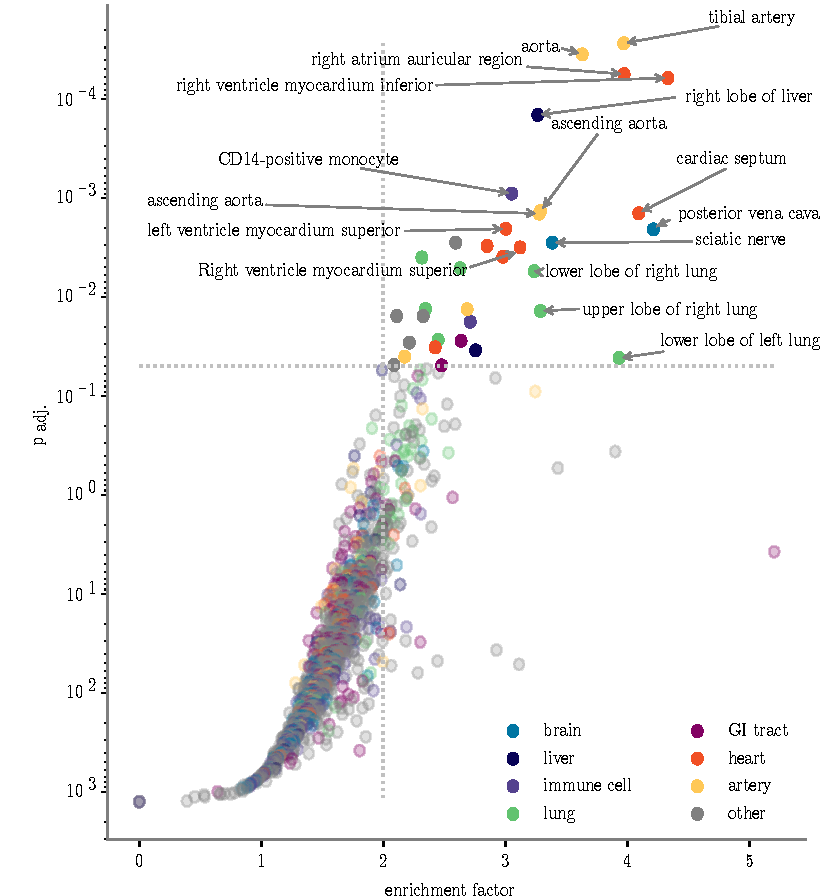
\includegraphics{Abbildung/enrichment_scatter.pdf}

	\begin{minipage}{\captionwidth}
		\caption[enrichemtn]{\uzlemph{Enrichment Analysis for overlap of \ac{cad} \ac{gwas} proxy variants with tissue specific \acp{cCRE}} \newline p-values and enrichment factors for the overlap of \ac{cad} \ac{gwas} proxy variants (and variants in \ac{ld}) and tissue specific \acp{cCRE}. For details please refer to section \ref{sec:enrichment}.}
		\label{fig:enrichment_scatter}
	\end{minipage}
\end{figure}

As seen in figure \ref{fig:enrichment}, statistically significant enrichment ($p_{adj.}<0.05$) was observed for 34 biosamples. Using the biosample annotations from Cellosaurus, these biosamples were assigned to their tissue of origin. The most prominent groups of origin tissues are the heart (8), the lungs (7), and arteries (6), as summarized in table \ref{tab:enriched_tissues}. Other tissues included the liver, the \ac{gi} tract, the brain, and immune cells (CD14+ monocytes).


\begin{table}[h!]
\capstart
\centering
\begin{minipage}{\captionwidth}
    \caption[enriched tissues]{\uzlemph{Tissues Found in the Enrichment Analysis} \newline Tissues of biosamples which show statitically significant overlap between \ac{cad} \ac{gwas} proxy variants (and variants in \ac{ld}) and \acp{cCRE}.}
    \label{tab:enriched_tissues}
\end{minipage}
\begin{tabular}{|c|c|}
    \hline
    tissue      & count in significant biosamples \\ \hline
    heart       & 8                               \\
    lung        & 7                               \\
    artery      & 6                               \\
    liver       & 2                               \\
    GI tract    & 2                               \\
    brain       & 2                               \\
    immune cell & 2                               \\
    other       & 5                               \\ \hline
    total       & 34                              \\ \hline
    \end{tabular}
\end{table}
